
\documentclass[table]{eecslides}

% \usecolortheme{RimouskiDark}

\usepackage[french]{babel}
\usepackage{lipsum}

\usepackage{hyperref}
\usepackage{xcolor}
\usepackage[round,authoryear]{natbib}
\usepackage[protrusion=true,expansion=true]{microtype}
\usepackage{xcolor}
\usepackage{tabularx}
\usepackage{bookman}  

\usepackage{graphicx}
\usepackage{caption}

\setlength{\extrarowheight}{3pt}

\title[]{Role of alternative stable states on Sugar maple range shift in reaction to climate change.}
\author[]{\color{white}  Steve Vissault}
\website{\color{white} \textit{s.vissault@yahoo.fr}}
\institute[\color{white} UQAR]{\color{white} \textbf{Research proposal \\
Université du Québec à Rimouski}}
\date{ \color{white} \today}

\setbeamersize{text margin left=1cm} 
\setbeamersize{text margin right=1cm} 
\setbeamersize{text margin top=0.1cm} 

\begin{document}

\begin{frame}[plain]
	\titlepage
\end{frame}


%%%%%%%%%%%%%%%%
\section{Introduction}
%%%%%%%%%%%%%%%%

\begin{frame}{Introduction}{Context}

\begin{columns}[c]
	\begin{column}{.4\paperwidth}
		\begin{figure}
			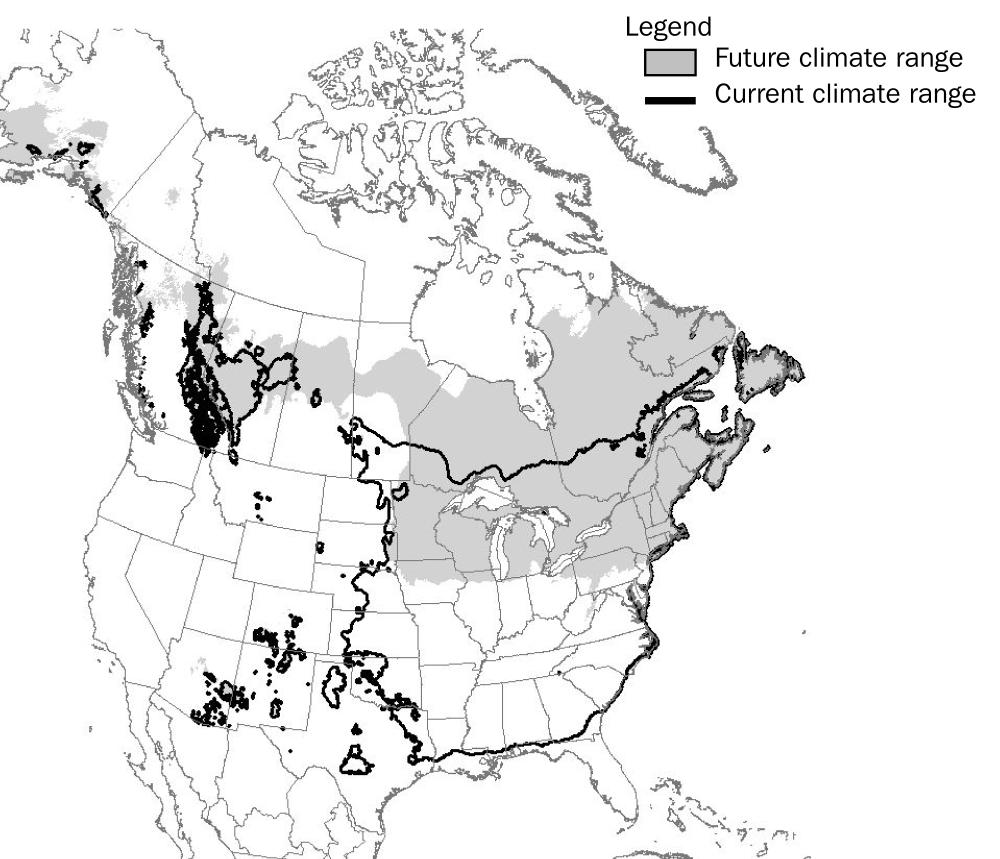
\includegraphics[width=.5\paperwidth]{sugar_map_distrib.jpg}
			\caption*{\scriptsize{\cite{Sciences2014}}}
		\end{figure}
	\end{column}
	\begin{column}{.5\paperwidth}
		 \begin{itemize}
		  \item Distribution of maple sugar is coming to shift northward
		  \item \textbf{Highly improbable: } Dispersal limitations and slow population dynamics.
		 \end{itemize}
	\end{column}
\end{columns}

\end{frame}



%%%%%%%%%%%%%%%%%%%%%%%%%%%%%%%%%%%%%%%%%%%%%%%%%%%%%%%%

%%%%%%%%%%%%%%%%
%% References
%%%%%%%%%%%%%%%%

\begin{frame}[allowsframebreaks]{Références}
	\scriptsize
	\bibliographystyle{abbrvnat}
	\bibliography{/home/steve/Dropbox/Bibtex/Devis}	
\end{frame}

\end{document}